Under vil vi diskutere funnene fra spørreundersøkelsen og dybdeintervjuene, og gjennom teori analysere resultatene opp mot problemstillingen. Til slutt vil vi gi anbefalinger relatert til hva virksomheten kan gjøre annerledes og områder ledelsen bør forbedre for å øke sannsynligheten for å nå virksomhetens mål.

\section{Konflikt mellom ledelsen og de ansatte}
Basert på intervjuene har vi identifisert uenighet mellom ledelsen og medarbeiderne med tanke på arbeidsmengden. Ledelsen mener at arbeidsmengden ikke oppleves som unormalt høy og at den er nødvendig for å levere resultatene de ønsker. De begrunner dette med et tøft marked hvor de må gripe prosjektmulighetene de får. I motsetning til ledelsen mener medarbeiderne at arbeidsmengden er for stor, og fører enkelte ganger til at de må utføre arbeidsoppgaver de ikke behersker godt nok. Ledelsen er ikke klar over at de ansatte mener arbeidsmengden er for stor, samtidig som at medarbeiderne tror ledelsen deler samme oppfatning som dem.

\begin{figure}[H]
\centering
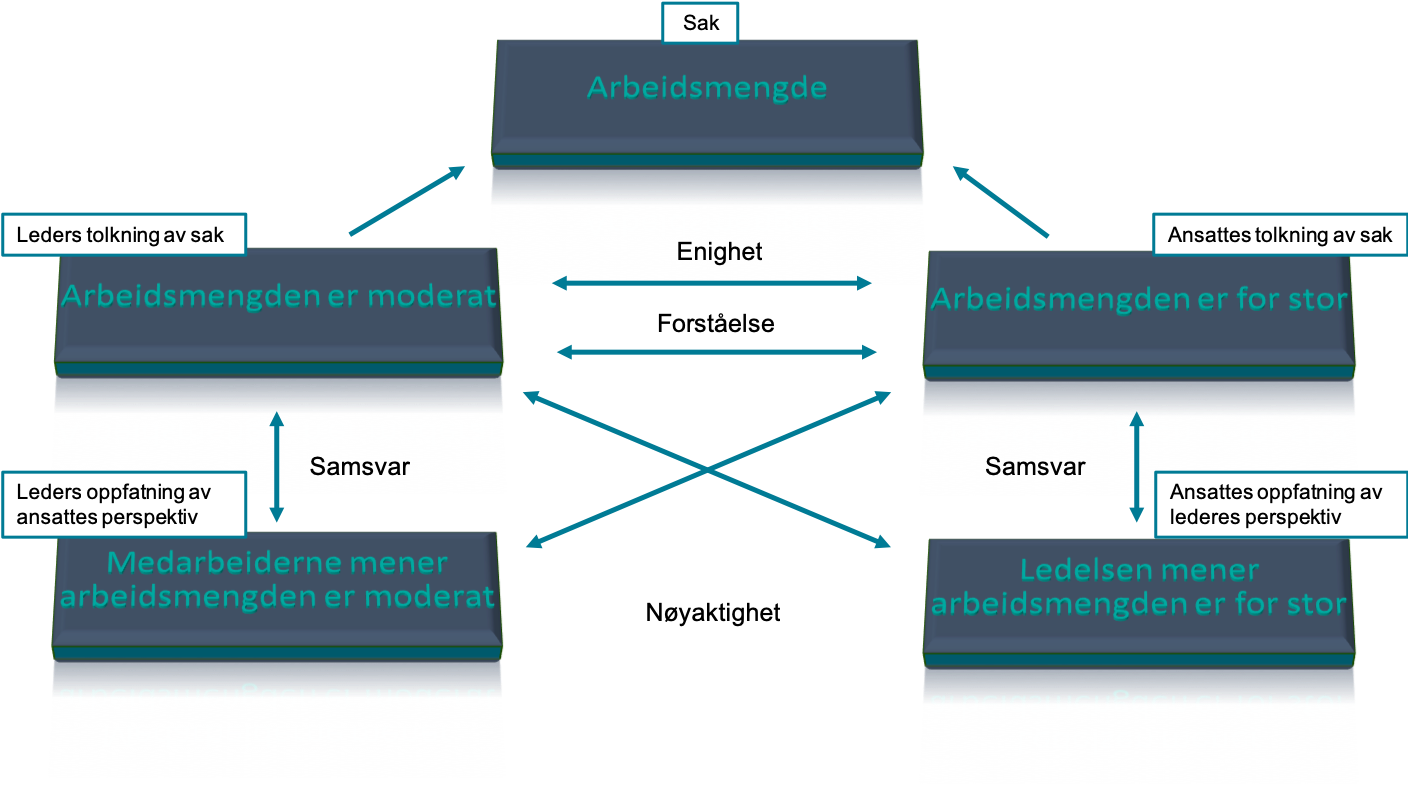
\includegraphics [scale=0.6]{bilder/koo.png}
\caption{Koorienteringsmodellen - arbeidsmengde}
\label{fig:koo}
\end{figure}

Koorienteringsmodellen viser at partene befinner seg i tilstanden som omtales som falsk konsensus. Den reflekterer én av to tilstander som tilsier at partene er i konflikt. Partene tror de er enige, men i virkeligheten er de uenige. I utgangspunktet er det positivt med utfordrende oppgaver, hvor lederen oppmuntrer de ansatte til kreativ problemløsning, og til å finne løsninger på problemer selv. Men i dette tilfellet føler medarbeiderne behov for hjelp og veiledning.

\indent \newline
Konflikten påvirker mestringsfølelsen hos de ansatte, og virker negativt inn på motivasjonen. En annen konsekvens er at det kan føre til at Involve leverer et svakere sluttprodukt til kundene. Dette kan påvirke lønnsomheten på sikt. På bakgrunn av analysen vil vi derfor oppfordre ledelsen til å tilbringe mer tid sammen med de ansatte, og veilede ved behov. 

\section{Manglende fokus på overordnet felles mål}
En av de viktigste oppgavene til en leder er å formidle felles mål og visjoner som sørger for at alle interessentene i virksomheten jobber mot det samme overordnede målet. Basert på vår analyse har ikke ledelsen klart å henge med i utviklingen innenfor kommunikasjonsbransjen, hvor mange av prosjektene krever samarbeid mellom avdelingene. Med for mye fokus på målsettinger innenfor hver avdeling, skapes det dårlige rammevilkår for et godt samarbeid mellom de ulike grupperingene i virksomheten. En slik suboptimalisering vil kunne føre til at de ansatte jobber mot resultater som vil gagne deres avdeling, men som ikke nødvendigvis er optimalt for virksomheten totalt sett. Ledelsen bør derfor definere en tydeligere visjon og felles målsetting, samtidig som hver enkelt avdelingsleder jobber med å kommunisere disse. Fokus på dette området vil kunne skape bedre forutsetninger for effektivt samarbeid og ansatte som jobber mot en felles retning og visjon. 

\section{Effektiv ledelse}
I oppgaven har vi definert ledelse som evnen til å skape oppslutning fra folk som prinsipielt kunne villet noe annet, og å mobilisere innsatsvilje og samarbeid mot et felles mål. I tillegg fant vi det hensiktsmessig å skille ledelse fra makt, styring og autoritet. For å avgjøre om Involve praktiserer effektiv ledelse i dag, har vi basert analysen vår på teori om transformasjonsledelse og transaksjonsledelse. Videre drøftelse vil først ta utgangspunkt i Bass sine fire dimensjoner som omhandler transformasjonslederens karisma, og til slutt transaksjonsledelse.

\subsection{Idealisert innflytelse}
Analysene viser til medarbeidere som er misfornøyde med arbeidsmengden. I relasjon til dette punktet opptrer lederne som gode rollemodeller i form av arbeidsinnsatsen de legger ned for organisasjonen. Derimot tilbringer lederne for lite tid med de ansatte og evner derfor ikke å skape innflytelse hos dem.

\subsection{Inspirerende motivasjon}
Ledelsen har et forbedringspotensial i henhold til å inspirere og motivere medarbeiderne gjennom å skape tilhørighet til felles mål og visjoner. Hovedutfordringen ligger i den strategiske kommunikasjonen relatert til målsettinger, i form av at det fokuseres for mye på målsettinger knyttet til hver enkelt avdeling. Samarbeid mellom avdelingene blir dermed vanskelig og en suboptimalisert virksomhet som resultat av dette, hvor hver avdeling blir motivert ut fra mål som ikke nødvendigvis samsvarer med hva som totalt sett er best for organisasjonen (skriv om).  

\subsection{Inspirerende motivasjon}
5.3.3 Intellektuell stimulering
Dimensjonen som omhandler lederens evne til å fremme kreativitet og innovativ atferd var den dimensjonen med høyest score i spørreundersøkelsen. Gjennom analysene våre kommer det frem at ledelsen er flinke til å gi de ansatte kreativt spillerom, uten å blande seg inn i utførelsen av prosjektene. Medarbeiderne savner imidlertid veiledning til å løse vanskelig oppgaver som de føler de ikke behersker godt nok.

\subsection{Inspirerende motivasjon}
5.3.4 Individuelle hensyn
I forhold til dimensjonen som omhandler samhandling med hver enkelt ansatt og deres behov for individuell måloppnåelse og vekst finner vi forbedringspotensiale for ledelsen. For mye tid brukes på eksterne interessenter, og lederne klarer dermed ikke å etablere personlige forhold til de ansatte. (også på dette punktet savner medarbeiderne læringsorientert veiledning/hjelp, skal vi skrive det her også?)

\subsection{Inspirerende motivasjon}
5.3.5 Transaksjonsledelse 
Analysene viser videre at ledelsen ikke har for vane å motivere de ansatte ved bruk av bonuser. I følge medarbeideren vi intervjuet, har ledelsen tidligere prøvd ut bonusordninger, men det har ikke blitt tatt godt i mot blant de ansatte.  Årsaken til dette er at det skapte konkurranse internt i virksomheten, i tillegg til at målene føltes uoppnåelige. Motivasjonen ble påvirket negativt og bonussystemet virket derfor mot sin hensikt. Bonussystemer kan i utgangspunktet fungere som et motivasjonsinsentiv. Hvis ledelsen ønsker å bruke dette, vil vi imidlertid anbefale å bruke team-baserte bonusordninger for å unngå og skape konkurranse mellom de ansatte.

\section{Anbefalinger}
5.4 Anbefalinger
Analysene viser at dagens utøvelse av ledelse er en mellomting av transformasjonsledelse, transaksjonsledelse og styring, med hovedvekt på de to sistnevnte ledelsesstilene. Lederne har for lite fokus på å skape personlige relasjoner med de ansatte, samt skape motivasjon og inspirasjon til å jobbe mot felles mål. For at Involve skal effektivisere ledelsen, og dermed potensielt forbedre mulighetene for å nå målsettingene, anbefaler vi følgende:
Utarbeide et tydelig overordnet mål som avdelingslederne sørger for å kommunisere jevnlig til medarbeiderne i hver enkelt avdeling.
Avsette mer tid sammen med de ansatte for å skape personlige relasjoner og lære om enkeltindividers personlige mål og behov for vekst.
Tilby hjelp og veiledning når medarbeiderne jobber med utfordrende oppgaver som tærer på motivasjon og mestringsfølelsen.
Eventuelle bonusordninger bør innføres på bakgrunn av team-baserte prestasjoner.
